

\tikzset{every picture/.style={line width=0.75pt}} %set default line width to 0.75pt        
\centering
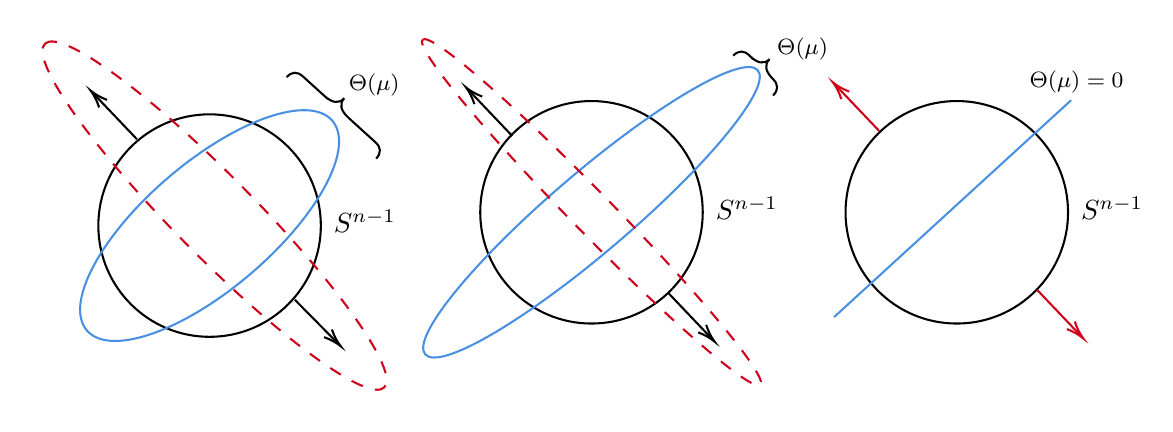
\begin{tikzpicture}[x=0.75pt,y=0.75pt,yscale=-0.8,xscale=0.8]
%uncomment if require: \path (0,302); %set diagram left start at 0, and has height of 302

%Shape: Circle [id:dp5978115037546095] 
\draw   (35,143.33) .. controls (35,106.33) and (65,76.33) .. (102,76.33) .. controls (139,76.33) and (169,106.33) .. (169,143.33) .. controls (169,180.33) and (139,210.33) .. (102,210.33) .. controls (65,210.33) and (35,180.33) .. (35,143.33) -- cycle ;
%Shape: Ellipse [id:dp29341954877000376] 
\draw  [color={rgb, 255:red, 74; green, 144; blue, 226 }  ,draw opacity=1 ] (28.08,206.46) .. controls (14.4,190.44) and (36.4,149.19) .. (77.23,114.32) .. controls (118.05,79.46) and (162.24,64.18) .. (175.92,80.2) .. controls (189.6,96.21) and (167.6,137.47) .. (126.77,172.33) .. controls (85.95,207.2) and (41.76,222.48) .. (28.08,206.46) -- cycle ;
%Shape: Ellipse [id:dp23881267719319044] 
\draw  [color={rgb, 255:red, 208; green, 2; blue, 27 }  ,draw opacity=1 ][dash pattern={on 4.5pt off 4.5pt}] (2.91,33.73) .. controls (12.74,24.77) and (66.42,63.88) .. (122.81,121.1) .. controls (179.19,178.32) and (216.93,231.97) .. (207.09,240.93) .. controls (197.26,249.89) and (143.58,210.77) .. (87.19,153.55) .. controls (30.81,96.34) and (-6.93,42.69) .. (2.91,33.73) -- cycle ;
%Straight Lines [id:da7441815125115865] 
\draw    (58.23,91.32) -- (31.71,63.45) ;
\draw [shift={(30.33,62)}, rotate = 46.43] [color={rgb, 255:red, 0; green, 0; blue, 0 }  ][line width=0.75]    (10.93,-3.29) .. controls (6.95,-1.4) and (3.31,-0.3) .. (0,0) .. controls (3.31,0.3) and (6.95,1.4) .. (10.93,3.29)   ;
%Shape: Circle [id:dp7005638453799473] 
\draw   (265,135.33) .. controls (265,98.33) and (295,68.33) .. (332,68.33) .. controls (369,68.33) and (399,98.33) .. (399,135.33) .. controls (399,172.33) and (369,202.33) .. (332,202.33) .. controls (295,202.33) and (265,172.33) .. (265,135.33) -- cycle ;
%Shape: Ellipse [id:dp6845662037057292] 
\draw  [color={rgb, 255:red, 74; green, 144; blue, 226 }  ,draw opacity=1 ] (231.85,220.86) .. controls (223.25,210.79) and (261.12,164.34) .. (316.43,117.1) .. controls (371.74,69.86) and (423.55,39.73) .. (432.15,49.79) .. controls (440.75,59.86) and (402.88,106.32) .. (347.57,153.56) .. controls (292.26,200.8) and (240.45,230.93) .. (231.85,220.86) -- cycle ;
%Shape: Ellipse [id:dp8539648982603185] 
\draw  [color={rgb, 255:red, 208; green, 2; blue, 27 }  ,draw opacity=1 ][dash pattern={on 4.5pt off 4.5pt}] (230.29,31.35) .. controls (235.31,26.81) and (284.92,69.68) .. (341.09,127.11) .. controls (397.26,184.53) and (438.73,234.76) .. (433.71,239.3) .. controls (428.69,243.84) and (379.08,200.97) .. (322.91,143.55) .. controls (266.74,86.13) and (225.27,35.9) .. (230.29,31.35) -- cycle ;
%Straight Lines [id:da14020280087178227] 
\draw    (284.23,89.32) -- (257.71,61.45) ;
\draw [shift={(256.33,60)}, rotate = 46.43] [color={rgb, 255:red, 0; green, 0; blue, 0 }  ][line width=0.75]    (10.93,-3.29) .. controls (6.95,-1.4) and (3.31,-0.3) .. (0,0) .. controls (3.31,0.3) and (6.95,1.4) .. (10.93,3.29)   ;
%Straight Lines [id:da5603361679448644] 
\draw    (378.33,184) -- (404.85,211.87) ;
\draw [shift={(406.23,213.32)}, rotate = 226.43] [color={rgb, 255:red, 0; green, 0; blue, 0 }  ][line width=0.75]    (10.93,-3.29) .. controls (6.95,-1.4) and (3.31,-0.3) .. (0,0) .. controls (3.31,0.3) and (6.95,1.4) .. (10.93,3.29)   ;
%Shape: Circle [id:dp9475784237826396] 
\draw   (485,135.33) .. controls (485,98.33) and (515,68.33) .. (552,68.33) .. controls (589,68.33) and (619,98.33) .. (619,135.33) .. controls (619,172.33) and (589,202.33) .. (552,202.33) .. controls (515,202.33) and (485,172.33) .. (485,135.33) -- cycle ;
%Straight Lines [id:da6044181775537695] 
\draw [color={rgb, 255:red, 208; green, 2; blue, 27 }  ,draw opacity=1 ]   (505.23,86.32) -- (478.71,58.45) ;
\draw [shift={(477.33,57)}, rotate = 46.43] [color={rgb, 255:red, 208; green, 2; blue, 27 }  ,draw opacity=1 ][line width=0.75]    (10.93,-3.29) .. controls (6.95,-1.4) and (3.31,-0.3) .. (0,0) .. controls (3.31,0.3) and (6.95,1.4) .. (10.93,3.29)   ;
%Straight Lines [id:da29508541854137216] 
\draw [color={rgb, 255:red, 208; green, 2; blue, 27 }  ,draw opacity=1 ]   (600.33,182) -- (626.85,209.87) ;
\draw [shift={(628.23,211.32)}, rotate = 226.43] [color={rgb, 255:red, 208; green, 2; blue, 27 }  ,draw opacity=1 ][line width=0.75]    (10.93,-3.29) .. controls (6.95,-1.4) and (3.31,-0.3) .. (0,0) .. controls (3.31,0.3) and (6.95,1.4) .. (10.93,3.29)   ;
%Straight Lines [id:da38477923288259275] 
\draw [color={rgb, 255:red, 74; green, 144; blue, 226 }  ,draw opacity=1 ]   (478.08,198.46) -- (620.82,67.86) ;
%Straight Lines [id:da7861012215950758] 
\draw    (153.33,188) -- (179.59,214.58) ;
\draw [shift={(181,216)}, rotate = 225.34] [color={rgb, 255:red, 0; green, 0; blue, 0 }  ][line width=0.75]    (10.93,-3.29) .. controls (6.95,-1.4) and (3.31,-0.3) .. (0,0) .. controls (3.31,0.3) and (6.95,1.4) .. (10.93,3.29)   ;
%Shape: Brace [id:dp7772620483523939] 
\draw   (202.33,103) .. controls (205.47,99.55) and (205.31,96.25) .. (201.85,93.11) -- (185.8,78.55) .. controls (180.87,74.07) and (179.97,70.1) .. (183.1,66.64) .. controls (179.97,70.1) and (175.93,69.59) .. (170.99,65.11)(173.21,67.12) -- (158.22,53.52) .. controls (154.77,50.39) and (151.47,50.55) .. (148.33,54) ;
%Shape: Brace [id:dp11747602823300118] 
\draw   (441.33,65) .. controls (444.62,61.71) and (444.62,58.41) .. (441.33,55.12) -- (441.33,55.12) .. controls (436.62,50.41) and (435.92,46.41) .. (439.22,43.12) .. controls (435.92,46.41) and (431.92,45.71) .. (427.22,41)(429.33,43.12) -- (427.22,41) .. controls (423.92,37.71) and (420.62,37.71) .. (417.33,41) ;

% Text Node
\draw (175,132.06) node [anchor=north west][inner sep=0.75pt]    {$\mathbb{S}^{n-1}$};
% Text Node
\draw (405,124.06) node [anchor=north west][inner sep=0.75pt]    {$\mathbb{S}^{n-1}$};
% Text Node
\draw (625,124.06) node [anchor=north west][inner sep=0.75pt]    {$\mathbb{S}^{n-1}$};
% Text Node
\draw (184,50.4) node [anchor=north west][inner sep=0.75pt]  [font=\footnotesize]  {$\Theta ( \mu )$};
% Text Node
\draw (442,28.4) node [anchor=north west][inner sep=0.75pt]  [font=\footnotesize]  {$\Theta ( \mu )$};
% Text Node
\draw (594,48.4) node [anchor=north west][inner sep=0.75pt]  [font=\footnotesize]  {$\Theta ( \mu ) =0$};


\end{tikzpicture}
